\documentclass[11pt]{article}

% ── Packages ──────────────────────────────────────────────────────────────────
\usepackage[margin=1in]{geometry}
\usepackage{amsmath, amssymb, amsthm}
\usepackage{mathtools}
\usepackage{xcolor}
\usepackage{mdframed}
\usepackage{enumitem}
\usepackage{hyperref}
\usepackage{pagecolor}
\usepackage{microtype}
\usepackage{tikz}
\usetikzlibrary{arrows.meta, positioning, shapes.geometric}

% ── Page colour (cream) ───────────────────────────────────────────────────────
\definecolor{cream}{HTML}{FFFDF5}
\definecolor{defblue}{HTML}{1A4A7A}
\definecolor{thmgreen}{HTML}{1A5C3A}
\definecolor{warnAmber}{HTML}{7A4A00}
\definecolor{dangerRed}{HTML}{7A1A1A}
\definecolor{boxbluebg}{HTML}{EBF3FB}
\definecolor{boxgreenbg}{HTML}{EBF7EF}
\definecolor{boxamberbg}{HTML}{FDF5E6}
\definecolor{boxredbg}{HTML}{FBEBEB}
\pagecolor{cream}

% ── Theorem environments ───────────────────────────────────────────────────────
\newtheoremstyle{defstyle}{8pt}{8pt}{\normalfont}{0pt}{\bfseries\color{defblue}}{.}{0.5em}{}
\newtheoremstyle{thmstyle}{8pt}{8pt}{\normalfont}{0pt}{\bfseries\color{thmgreen}}{.}{0.5em}{}
\newtheoremstyle{notstyle}{8pt}{8pt}{\normalfont}{0pt}{\bfseries\color{warnAmber}}{.}{0.5em}{}
\newtheoremstyle{cautionstyle}{8pt}{8pt}{\normalfont}{0pt}{\bfseries\color{dangerRed}}{.}{0.5em}{}

\theoremstyle{defstyle}
\newtheorem{definition}{Definition}[section]

\theoremstyle{thmstyle}
\newtheorem{theorem}{Theorem}[section]

\theoremstyle{notstyle}
\newtheorem*{remark}{Remark}
\newtheorem*{example}{Example}

\theoremstyle{cautionstyle}
\newtheorem*{caution}{Caution}

% ── Coloured framed boxes ──────────────────────────────────────────────────────
\newmdenv[
  backgroundcolor=boxbluebg, linecolor=defblue, linewidth=2pt,
  topline=false, rightline=false, bottomline=false,
  innerleftmargin=10pt, innerrightmargin=10pt,
  innertopmargin=6pt, innerbottommargin=6pt,
  skipabove=8pt, skipbelow=8pt
]{defbox}

\newmdenv[
  backgroundcolor=boxgreenbg, linecolor=thmgreen, linewidth=2pt,
  topline=false, rightline=false, bottomline=false,
  innerleftmargin=10pt, innerrightmargin=10pt,
  innertopmargin=6pt, innerbottommargin=6pt,
  skipabove=8pt, skipbelow=8pt
]{thmbox}

\newmdenv[
  backgroundcolor=boxamberbg, linecolor=warnAmber, linewidth=2pt,
  topline=false, rightline=false, bottomline=false,
  innerleftmargin=10pt, innerrightmargin=10pt,
  innertopmargin=6pt, innerbottommargin=6pt,
  skipabove=8pt, skipbelow=8pt
]{notebox}

\newmdenv[
  backgroundcolor=boxredbg, linecolor=dangerRed, linewidth=2pt,
  topline=false, rightline=false, bottomline=false,
  innerleftmargin=10pt, innerrightmargin=10pt,
  innertopmargin=6pt, innerbottommargin=6pt,
  skipabove=8pt, skipbelow=8pt
]{cautionbox}

% ── Macros ────────────────────────────────────────────────────────────────────
\newcommand{\Z}{\mathbb{Z}}
\newcommand{\N}{\mathbb{N}}
\newcommand{\R}{\mathbb{R}}

% ── Document ──────────────────────────────────────────────────────────────────
\begin{document}

\begin{center}
  {\Large\bfseries Lecture 26 --- Injective and Surjective Functions}\\[4pt]
  {\normalsize CS 173: Discrete Structures \quad$\cdot$\quad Functions}\\[2pt]
  {\small\color{gray} University of Illinois at Urbana-Champaign}
\end{center}

\vspace{1em}
\hrule
\vspace{1.5em}

% ══════════════════════════════════════════════════════════════════════════════
\section{Setup}

Throughout this lecture, let $A$ and $B$ be sets and let $f : A \to B$ be a function.

% ══════════════════════════════════════════════════════════════════════════════
\section{Injective Functions (Injections)}

\begin{defbox}
\begin{definition}[Injective function / injection]
$f$ is \emph{injective} (also called a \emph{one-to-one function} or an \emph{injection}) if and only if
\[
  \forall\, a_1, a_2 \in A,\quad f(a_1) = f(a_2) \;\Rightarrow\; a_1 = a_2.
\]
Equivalently, using the contrapositive:
\[
  a_1 \neq a_2 \;\Rightarrow\; f(a_1) \neq f(a_2).
\]
That is, distinct inputs always map to distinct outputs.
\end{definition}
\end{defbox}

\begin{notebox}
\begin{remark}
The two formulations are logically equivalent by contraposition:
\[
  \bigl(f(a_1) = f(a_2) \Rightarrow a_1 = a_2\bigr)
  \;\iff\;
  \bigl(a_1 \neq a_2 \Rightarrow f(a_1) \neq f(a_2)\bigr).
\]
The contrapositive form is often more intuitive: no two different inputs share the same output.
\end{remark}
\end{notebox}

\subsection*{Diagram: Injection vs.\ Non-injection}

\begin{center}
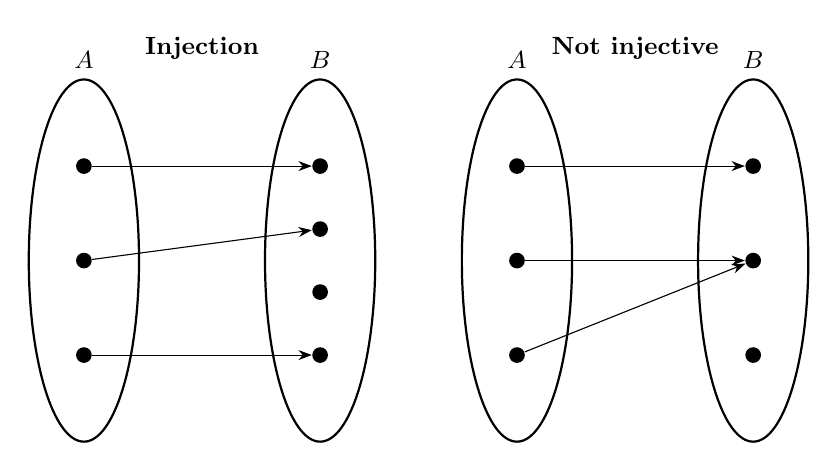
\begin{tikzpicture}[
    every node/.style={font=\small},
    dot/.style={circle, fill, inner sep=2pt},
    >=Stealth
  ]

  % ── Injection (left) ────────────────────────────────────────────────────
  % Oval: centre y=1, semi-height 2.3cm  →  y range [-1.3, 3.3]
  % 3-dot sets: y = 2.2, 1.0, -0.2   (well inside the [-1.3,3.3] range)
  % 4-dot sets: y = 2.2, 1.4, 0.6, -0.2
  \begin{scope}[xshift=0cm]
    \node[font=\bfseries\small] at (1.5, 3.7) {Injection};

    \draw[thick] (0, 1) ellipse (0.7cm and 2.3cm);
    \node at (0, 3.55) {$A$};
    \node[dot] (a1) at (0,  2.2) {};
    \node[dot] (a2) at (0,  1.0) {};
    \node[dot] (a3) at (0, -0.2) {};

    \draw[thick] (3, 1) ellipse (0.7cm and 2.3cm);
    \node at (3, 3.55) {$B$};
    \node[dot] (b1) at (3,  2.2) {};
    \node[dot] (b2) at (3,  1.4) {};
    \node[dot] (b3) at (3,  0.6) {};
    \node[dot] (b4) at (3, -0.2) {};

    \draw[->] (a1) -- (b1);
    \draw[->] (a2) -- (b2);
    \draw[->] (a3) -- (b4);
    % b3 is not mapped to — valid for injection
  \end{scope}

  % ── Non-injection (right) ───────────────────────────────────────────────
  \begin{scope}[xshift=5.5cm]
    \node[font=\bfseries\small] at (1.5, 3.7) {Not injective};

    \draw[thick] (0, 1) ellipse (0.7cm and 2.3cm);
    \node at (0, 3.55) {$A$};
    \node[dot] (c1) at (0,  2.2) {};
    \node[dot] (c2) at (0,  1.0) {};
    \node[dot] (c3) at (0, -0.2) {};

    \draw[thick] (3, 1) ellipse (0.7cm and 2.3cm);
    \node at (3, 3.55) {$B$};
    \node[dot] (d1) at (3,  2.2) {};
    \node[dot] (d2) at (3,  1.0) {};
    \node[dot] (d3) at (3, -0.2) {};

    % c2 and c3 both map to d2 — violates injectivity
    \draw[->] (c1) -- (d1);
    \draw[->] (c2) -- (d2);
    \draw[->] (c3) -- (d2);
  \end{scope}

\end{tikzpicture}
\end{center}

% ══════════════════════════════════════════════════════════════════════════════
\section{Surjective Functions (Surjections)}

\begin{defbox}
\begin{definition}[Surjective function / surjection]
$f$ is \emph{surjective} (also called \emph{onto} or a \emph{surjection}) if and only if
\[
  \forall\, y \in B,\quad \exists\, x \in A,\quad f(x) = y.
\]
That is, every element of the codomain $B$ is the image of \emph{at least one} element of $A$.
\end{definition}
\end{defbox}

\begin{notebox}
\begin{remark}
Surjectivity is a property of the \emph{codomain}: it says that $f$ ``hits'' every element of $B$.  A function can be surjective without being injective (multiple inputs can share the same output, as long as no output is left uncovered).
\end{remark}
\end{notebox}

\subsection*{Diagram: Surjection vs.\ Non-surjection}

\begin{center}
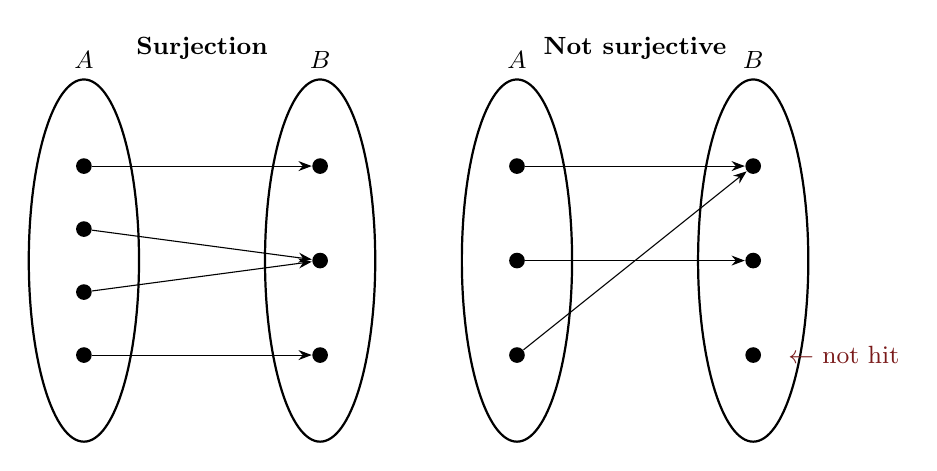
\begin{tikzpicture}[
    every node/.style={font=\small},
    dot/.style={circle, fill, inner sep=2pt},
    >=Stealth
  ]

  % ── Surjection (left) ───────────────────────────────────────────────────
  \begin{scope}[xshift=0cm]
    \node[font=\bfseries\small] at (1.5, 3.7) {Surjection};

    % Domain: 4 dots
    \draw[thick] (0, 1) ellipse (0.7cm and 2.3cm);
    \node at (0, 3.55) {$A$};
    \node[dot] (a1) at (0,  2.2) {};
    \node[dot] (a2) at (0,  1.4) {};
    \node[dot] (a3) at (0,  0.6) {};
    \node[dot] (a4) at (0, -0.2) {};

    % Codomain: 3 dots
    \draw[thick] (3, 1) ellipse (0.7cm and 2.3cm);
    \node at (3, 3.55) {$B$};
    \node[dot] (b1) at (3,  2.2) {};
    \node[dot] (b2) at (3,  1.0) {};
    \node[dot] (b3) at (3, -0.2) {};

    \draw[->] (a1) -- (b1);
    \draw[->] (a2) -- (b2);
    \draw[->] (a3) -- (b2);
    \draw[->] (a4) -- (b3);
  \end{scope}

  % ── Non-surjection (right) ──────────────────────────────────────────────
  \begin{scope}[xshift=5.5cm]
    \node[font=\bfseries\small] at (1.5, 3.7) {Not surjective};

    % Domain: 3 dots
    \draw[thick] (0, 1) ellipse (0.7cm and 2.3cm);
    \node at (0, 3.55) {$A$};
    \node[dot] (c1) at (0,  2.2) {};
    \node[dot] (c2) at (0,  1.0) {};
    \node[dot] (c3) at (0, -0.2) {};

    % Codomain: 3 dots; bottom one never hit
    \draw[thick] (3, 1) ellipse (0.7cm and 2.3cm);
    \node at (3, 3.55) {$B$};
    \node[dot] (d1) at (3,  2.2) {};
    \node[dot] (d2) at (3,  1.0) {};
    \node[dot] (d3) at (3, -0.2) {};

    \draw[->] (c1) -- (d1);
    \draw[->] (c2) -- (d2);
    \draw[->] (c3) -- (d1);
    \node[color=dangerRed, font=\small] at (4.15, -0.2) {$\leftarrow$ not hit};
  \end{scope}

\end{tikzpicture}
\end{center}

% ══════════════════════════════════════════════════════════════════════════════
\section{Comparing Injection and Surjection}

\begin{center}
\renewcommand{\arraystretch}{1.5}
\begin{tabular}{|l|l|l|}
\hline
\textbf{Property} & \textbf{Injective} & \textbf{Surjective} \\
\hline
Formal statement
  & $f(a_1)=f(a_2) \Rightarrow a_1=a_2$
  & $\forall y\in B,\;\exists x\in A,\; f(x)=y$ \\
Informal meaning
  & No two inputs share an output
  & Every output is reachable \\
Constraint on
  & \emph{inputs} (domain $A$)
  & \emph{outputs} (codomain $B$) \\
Violations
  & Two arrows into one dot in $B$
  & A dot in $B$ with no arrow \\
\hline
\end{tabular}
\end{center}

% ══════════════════════════════════════════════════════════════════════════════
\section{Bijections}

\begin{defbox}
\begin{definition}[Bijection]
$f : A \to B$ is a \emph{bijection} (or \emph{one-to-one correspondence}) if it is both injective and surjective:
\[
  f \text{ is bijective} \;\iff\; f \text{ is injective} \;\wedge\; f \text{ is surjective}.
\]
\end{definition}
\end{defbox}

\begin{notebox}
\begin{remark}
A bijection pairs every element of $A$ with exactly one element of $B$ and vice versa.  Bijections are precisely the functions that have a well-defined inverse $f^{-1}: B \to A$.
\end{remark}
\end{notebox}

% ══════════════════════════════════════════════════════════════════════════════
\section{Cardinality}

\subsection{Comparing the sizes of sets}

Given sets $A$ and $B$, we compare their cardinalities using injections and surjections — this works even for infinite sets where direct counting is impossible.

\begin{defbox}
\begin{definition}[$|A| \leq |B|$]
The \emph{cardinality of $A$ is less than or equal to the cardinality of $B$}, written $|A| \leq |B|$, if and only if there exists an injective function from $A$ to $B$:
\[
  |A| \leq |B| \;\iff\; \exists\, f\bigl(\,f : A \to B \;\wedge\; f \text{ is injective}\bigr).
\]
\end{definition}
\end{defbox}

\begin{defbox}
\begin{definition}[$|A| \geq |B|$]
The \emph{cardinality of $A$ is greater than or equal to the cardinality of $B$}, written $|A| \geq |B|$, if and only if there exists a surjective function from $A$ to $B$:
\[
  |A| \geq |B| \;\iff\; \exists\, f\bigl(\,f : A \to B \;\wedge\; f \text{ is surjective}\bigr).
\]
\end{definition}
\end{defbox}

\begin{notebox}
\begin{remark}
The asymmetry is intuitive: an injection $A \hookrightarrow B$ ``fits'' all of $A$ into $B$ without collisions, so $B$ must be at least as large.  A surjection $A \twoheadrightarrow B$ ``covers'' all of $B$ from $A$, so $A$ must be at least as large.
\end{remark}
\end{notebox}

\subsection{Equal cardinality}

\begin{defbox}
\begin{definition}[$|A| = |B|$]
$A$ and $B$ have the \emph{same cardinality}, written $|A| = |B|$, if and only if \emph{all three} of the following equivalent conditions hold:
\begin{align*}
  |A| = |B|
  &\;\iff\; \exists\, f\bigl(\,f : A \to B \;\wedge\; f \text{ is injective}\bigr)
             \;\wedge\;
             \exists\, g\bigl(\,g : A \to B \;\wedge\; g \text{ is surjective}\bigr) \\[4pt]
  &\;\iff\; \exists\, f\bigl(\,f : A \to B \;\wedge\; f \text{ is bijective}\bigr).
\end{align*}
That is, $|A|=|B|$ means both $|A| \leq |B|$ and $|A| \geq |B|$, which is equivalent to the existence of a bijection.
\end{definition}
\end{defbox}

\begin{thmbox}
\begin{theorem}[Cantor--Schr\"{o}der--Bernstein]
\[
  \forall x\, \forall y\,\Bigl(\bigl(|x| \leq |y| \;\wedge\; |y| \leq |x|\bigr) \;\Rightarrow\; |x| = |y|\Bigr).
\]
That is, if there exist injections $f: x \to y$ and $g: y \to x$, then there exists a bijection between $x$ and $y$.
\end{theorem}
\end{thmbox}

\begin{notebox}
\begin{remark}[This is one direction only]
The theorem is stated as $\Rightarrow$, not $\iff$.  The converse direction —
\[
  |x| = |y| \;\Rightarrow\; |x| \leq |y| \;\wedge\; |y| \leq |x|
\]
— is \emph{trivially true by definition}: since $|x|=|y|$ means a bijection $f: x \to y$ exists, and a bijection is both injective and surjective, we immediately get injections in both directions.  The non-trivial, hard direction is the one the theorem proves: that \emph{two injections} (which need not be inverses of each other) are sufficient to guarantee a bijection exists.
\end{remark}
\end{notebox}

\subsection{Summary table}

\begin{center}
\renewcommand{\arraystretch}{1.6}
\begin{tabular}{|c|l|l|}
\hline
\textbf{Notation} & \textbf{Meaning} & \textbf{Witness required} \\
\hline
$|A| \leq |B|$ & $A$ is no larger than $B$ & injective $f: A \to B$ \\
$|A| \geq |B|$ & $A$ is no smaller than $B$ & surjective $f: A \to B$ \\
$|A| = |B|$ & $A$ and $B$ are the same size & injection \emph{and} surjection $A \to B$; \\
             &                               & equivalently, bijection $f: A \to B$ \\
\end{tabular}
\end{center}

% ══════════════════════════════════════════════════════════════════════════════
\section{Summary}

\begin{enumerate}[leftmargin=*, label=\arabic*.]
  \item \textbf{Injection}: $\forall a_1, a_2 \in A,\; f(a_1) = f(a_2) \Rightarrow a_1 = a_2$.
  \item \textbf{Surjection}: $\forall y \in B,\; \exists x \in A,\; f(x) = y$.
  \item \textbf{Bijection}: injective $\wedge$ surjective.
  \item $|A| \leq |B| \iff \exists$ injective $f: A \to B$.
  \item $|A| \geq |B| \iff \exists$ surjective $f: A \to B$.
  \item $|A| = |B| \iff \exists$ injective $f: A\to B$ $\wedge$ $\exists$ surjective $g: A \to B$ $\iff$ $\exists$ bijection $f: A \to B$.
\end{enumerate}

\begin{notebox}
\begin{remark}[Looking ahead]
We will use injections and surjections to compare the sizes of infinite sets (cardinality) and define countability.
\end{remark}
\end{notebox}

\end{document}